%%%%%%%%%%%%%%
%%  Template for latex documents
%%  Author: Marco A. Aquino-Lopez
%%  Nota: to get a word document use pandoc
%%  pandoc -f latex Articulo.tex -o Articulo.docx --bibliography=bibliography.bib
%%%%%%%%%%%%%%%%%
%\documentclass [twocolumn,10pt] {article}
\documentclass [10pt] {article}

\usepackage [utf8] {inputenc}
\usepackage[english]{babel}

\usepackage {graphicx}
%\usepackage {amsfonts,unicode-math}
\usepackage {amsthm}
\usepackage {amsmath}
\usepackage {natbib}

\usepackage{hyperref}
\usepackage[in]{fullpage} %To have more in the page
%.____         ___________    ____  ___ 
%|    |   _____\__    _______ \   \/  / 
%|    |   \__  \ |    |_/ __ \ \     /  
%|    |___ / __ \|    |\  ___/ /     \  
%|_______ (____  |____| \___  /___/\  \ 
%        \/    \/           \/      \_/ 

\graphicspath{{Figures/}} %Setting the graphicspath

%Extra packages2
\usepackage{placeins}

%%%%%%

\date{ }
\usepackage{color}

%%%% To mark notes or added text by Author1 (a1)
%%%% This allows to add notes
%\newcommand{\a1}{\color{red} }  %% begin
%\newcommand{\1a}{ \color{black}} %% end
%\newcommand{\cuta1}[1]{\ac [cut] \ca} %% to mark cut text
%\newcommand{\notea1}[1]{\textcolor{red}{(note)}\footnote{\ac #1 \ca}}  %% To add a note or comment

% %%%% To mark notes or added text by Andres (ac)
 \newcommand{\ac}{\color{red} }  %% begin
 \newcommand{\ca}{\color{black}} %% end
 \newcommand{\cutac}[1]{\ac [cut] \ca} %% to mark cut text
 \newcommand{\noteac}[1]{\textcolor{red}{(note)}\footnote{\ac #1 \ca}}  %% To add a note or comment

% %%%% To mark notes or added text by Marco (ma)
% \newcommand{\ma}{\color{blue} }  %% begin
% \newcommand{\am}{\color{black}} %% end
% \newcommand{\cutma}[1]{\ac [cut] \ca} %% to mark cut text
% \newcommand{\noteam}[1]{\textcolor{red}{(note)}\footnote{\ac #1 \ca}}  %% To add a note or comment


% NOTE: To produce blinded version, replace "0" with "1" below.
\newcommand{\blind}{1}
\newcommand{\papertitle}{
	Evaluation of $^{210}$Pb dating models using simulated datasets
 %A simulation study to compare $^{210}$Pb dating analyses 
}

\begin{document}
	\def\spacingset#1{\renewcommand{\baselinestretch}%
		{#1}\small\normalsize} \spacingset{1}
	%%%%%%%%%%%%%%%%%%%%%%%%%%%%%%%%%%%%%%%%%%%%%%%%%%%%%%%%%%%%%%%%%%%%%%%%%%%%%%
	\if1\blind
	{
		\title{\textbf{\papertitle}}

		\author{Marco A Aquino-L\'opez\thanks{
				Department of Geography, University of Cambridge, 
				Cambridge, United Kingdom
				email: \texttt{aquino@cimat.mx} } \thanks{Corresponding author.}
					\and
			Nicole K. Sanderson\thanks{
				GEOTOP Research Centre, Université du Québec à Montréal, 
				Montréal, Québec, H2X 3Y7, Canada. 
				email: \texttt{sanderson.nicole@uqam.ca}}
					\and
			Maarten Blaauw\thanks{School of Natural and Built Environment,
				Queen's University Belfast,
				Belfast, BT7-1NN, UK.
				email:\texttt{maarten.blaauw@qub.ac.uk}  }
					\and
			Joan-Albert Sanchez-Cabeza\thanks{
				Unidad Acad\'emica Mazatl\'an, 
				Instituto de Ciencias del Mar y Limnolog\'ia, 
				Universidad Nacional Aut\'onoma de Mexico, 
				82040 Mazatl\'an, M\'exico.
				email:\texttt{jasanchez@cmarl.unam.mx}} 
					\and
			Ana Carolina Ruiz-Fernandez\thanks{
				Unidad Acad\'emica Mazatl\'an, 
				Instituto de Ciencias del Mar y Limnolog\'ia, 
				Universidad Nacional Aut\'onoma de Mexico, 
				82040 Mazatl\'an, M\'exico.
				email:\texttt{caro@ola.icmyl.unam.mx}} 
					\and
			J Andr\'es Christen\thanks{
				Centro de Investigaci\'on en Matem\'aticas (CIMAT),
				Jalisco s/n, Valenciana, 36023 Guanajuato, Gto, Mexico.
				email: \texttt{jac@cimat.mx}  }
			}
		\maketitle
	} \fi

	\if0\blind
	{
		\bigskip
		\bigskip
		\bigskip
		\begin{center}
			{\LARGE\bf \papertitle}
		\end{center}
		\medskip
	} \fi
\bigskip

\begin{abstract}
The focus on understanding anthropogenic impacts on the environment has resulted in a significant number of studies on sedimentary records for the last $\sim$ 100-200 years. However, radiocarbon ($^{14}$C) dating, the most commonly used dating technique, suffers from poor resolution and large errors, complicating the dating of this period.
To overcome this limitation, sediment $^{210}$Pb (lead-210) dating has been widely adopted as it provides absolute and continuous dates for the last $\sim$ 100-150 years. However, the Constant Rate of Supply (CRS, or Constant Flux - CF) model, which relies on the radioactive decay equation as an age-depth relationship, limits the accuracy of the model used to approximate dates.

	In this paper, we compare the classical approach to $^{210}$Pb dating (CRS) with \textit{Plum}, a recently developed Bayesian approach for analyzing sedimentary $^{210}$Pb measurements. We generate simulated depth $^{210}$Pb profiles according to three different sedimentation processes and analyze them using both methods.
	It is important to note that different laboratories use varying approaches to apply the CRS model. Our results indicate that even with high dating resolution of the sediment record, the CRS model used in a non-expert mode fails to capture the true age values and does not improve in accuracy as more information becomes available. Conversely, \textit{Plum} consistently provides more accurate results even with relatively small sample sizes and demonstrates improved accuracy and precision with additional information.
\end{abstract}
	\noindent%
	{\it Keywords:} Plum, Age-depth models, Chronology, Constant Rate of Supply, Simulations, Comparison.
	\vfill
	\newpage
	\spacingset{1.45} % DON'T change the spacing!

%%%%%%%%%%%%%%%%%%%%%%%%%%%%%%%%%%%%%%%%%%%%%%%%%%%%%%%%%%%%%
%%%%%%%%%%%%%%%%%%%%%%%%%%%%%%%%%%%%%%%%%%%%%%%%%%%%%%%%%%%%%
\section{Introduction}

	Lead-210 ($^{210}$Pb) is a naturally occurring radioactive isotope that is part of the $^{238}$U decay chain and is formed in both the atmosphere and sediments. This isotope, with a half-life of 22.23 $\pm$ 0.12 years, is commonly used to date recently accumulated sediments ($<150$ years) and has become increasingly popular in recent decades for palaeoecological and pollution studies aimed at evaluating human impacts on the environment \citep[e.g.,][]{Courtney2019}. The accuracy of chronologies is critical in these environmental studies to correctly assign dates to geological, chemical, biological and ecological changes. Unlike other dating techniques such as radiocarbon dating, dating a single sediment layer using a single, independent $^{210}$Pb measurement is not possible. Instead, $^{210}$Pb activity is measured at different depths along a core (e.g., lake, peatland, marine sediments). A $^{210}$Pb-chronology can only be established under certain assumptions regarding the sedimentation process and when a suitable portion of the excess, or unsupported $^{210}$Pb decay curve is measured, which represents the total inventory from deposition (atmospheric or water column $^{210}$Pb) and runoff. It is important to note that the analysis of a complete series (data set) of $^{210}$Pb measurements must be carried out in order to obtain meaningful dates, as discussed by \citet{Aquino2018}.


	% A range of traditional data analyses, so called ``models'', are available for dating recent sediments using $^{210}$Pb; e.g. the Constant Initial Concentration \citep[CIC,][]{Goldberg1963}, also known as Constant Activity \citep[CA,][]{Robbins1975}, the Constant Flux : Constant sedimentation \citep[CF:CS,][]{Crozaz1964} and the Constant Rate of Supply  \citep[CRS,][]{Appleby1978,Robbins1978,Sanchez-Cabeza2012} also known as the Constant Flux model (CF). 
% The main assumption of the CIC model is that sediments have a constant initial $^{210}$Pb concentration. 
% Both CF:CS and CRS models assume a constant flux of $^{210}$Pb, but the CF:CS model also assumes that the sedimentation rate is constant. 
% The CRS model is by far the most popular (see Figure \ref{fig:210models}) and allows for estimating variable mass accumulation rates.
% The flexibility of the CRS model, in terms of its assumptions, comes at the cost of needing to measure a sufficient portion of the excess $^{210}$Pb inventory or the use of interpolation/extrapolation in order to properly estimate the complete inventory of $^{210}$Pb in the sediment. 


Several traditional data analysis models are available for dating recent sediments using $^{210}$Pb. These include the Constant Initial Concentration (CIC) model, also known as Constant Activity (CA) \citep{Goldberg1963, Robbins1975}, the Constant Flux : Constant Sedimentation (CF:CS) model \citep{Crozaz1964}, and the Constant Rate of Supply (CRS) model, also known as the Constant Flux model (CF) \citep{Appleby1978, Robbins1978, Sanchez-Cabeza2012}. The CIC model assumes that sediments have a constant initial $^{210}$Pb concentration, while both the CF:CS and CRS models assume a constant flux of $^{210}$Pb. The CF:CS model also assumes a constant sedimentation rate. Of these models, the CRS model is the most popular, as it allows for the estimation of variable mass accumulation rates (see Figure \ref{fig:210models}). However, the flexibility of the CRS model in terms of its assumptions comes at a cost, as it requires the measurement of a sufficient portion of the excess $^{210}$Pb inventory or the use of interpolation/extrapolation in order to estimate the complete inventory of $^{210}$Pb in the sediment.



\begin{figure}[h!]
	\begin{centering}
		\includegraphics[width=.75\linewidth]{barras.pdf}
		\caption{Frequency of $^{210}$Pb dating models used in papers between 1964 and 2017. Data gathered by \citet{Courtney2019} from a literature review of 271 papers. The models include the CF:CS \citep[Constant Flux - Constant Sedimentation;][]{Robbins1978}, CIC (Constant Initial Concentration) \citep{Goldberg1963,Crozaz1964,Robbins1978} and CRS  \citep[Constant Rate of Supply;][]{Appleby1978,Robbins1978}. }
		\label{fig:210models}
	\end{centering}
\end{figure}

%Caro quiere que este párrafo se integre al párrafo donde se habla de las modificaciones revisar después  
% moverlo a otra parte 
In recent years, the CRS model has undergone several modifications aimed at enhancing its accuracy and practicality \citep{Binford1990,Appleby2001,Sanchez-Cabeza2014}. These modifications can be classified into two categories: (1) improvements in the model's uncertainty quantification and (2) adjustments to the model's application when additional information is available, such as the presence of external dating markers like $^{137}$Cs profiles, laminated sediments, tephras, and contaminated layers that correspond to known sedimentary events \citep{Appleby1998,Appleby2001,Appleby2008}.


	A recent inter-laboratory model comparison experiment \citep{Barsanti2020} presented concerning results when it comes to producing consistent chronologies.
Two measured $^{210}$Pb datasets were sent to 14 laboratories around the world, these laboratories having varying degrees of expertise.
Each laboratory was asked to provide a chronology, given the same data. 
It is important to note that each laboratory applied their preferred model; in most cases the CRS model was used.
This experiment resulted in a wide range of chronologies, independently of the model used, providing different results even when the same model and dataset were used.
The authors reinforced the need to use independent time markers (independent dating sources) to validate and ``anchor" the chronologies, as suggested previously by \citet{Smith2001}.  
This comparison experiment clearly and critically shows the impact that user decisions and expert adaptations/revisions have on the resulting chronologies.
In order to replicate and/or update any given chronology, documenting such user decisions becomes extremely important, as is providing raw data; however raw data sets and user decisions are rarely reported.

In recent years, \citet{Aquino2018} introduced a Bayesian approach to $^{210}$Pb dating, named the \textit{Plum} model, as an alternative to the classical models. In this approach, every data point is considered to originate from a forward model that takes into account both the sedimentation process and the radioactive decay process. The \textit{Plum} model also assumes a constant flux of excess $^{210}$Pb to the sediment, similar to the CRS model, although this assumption can be relaxed at the expense of computational power. One important difference between the two models is that the \textit{Plum} model includes the supported $^{210}$Pb, which is a naturally occurring component in sediments and is usually treated as a hindrance variable.

	\citet{Blaauw2018} presented a comparison between classical and Bayesian age-depth models construction, both for real and simulated $^{14}$C-dated cores.
They concluded that Bayesian age-depth models provide a more accurate result and more realistic uncertainties under a wide range of scenarios.  
The objective of the present study is to test whether similar results are maintained in a more complex modelling situation, such as the construction of $^{210}$Pb-based age-depth models.
To do so, we compare $^{210}$Pb dates (accuracy) and uncertainties (precision) from the widely applied CRS model against \textit{Plum} using simulated cores, i.e. sedimentation ``scenarios''.
We also aim to observe the learning process of each of the models and estimate the amount of information needed to obtain a reasonable chronology for each model.
This process is of critical importance as the amount of information depends on the number of samples, which in turn depends on the budget, time and user decision of resources allocated to developing the age-depth model. 


%Esto debe ser revisado antes de tener una version final, se esta agregando una sección
	The paper is organized as follows: 
Section 2 provides a short introduction to the CRS model which is the most widely used, as well as \textit{Plum}.
Section 3 discusses the consideration and the experimental setup.
Section 4 presents the tools we use for the model comparison, describing the three different sedimentation scenario simulations.
Section 5 compares results for the overall chronologies and for single depths.
Lastly, Section 6 presents the conclusions and discussion of the results obtained in section 5. 

\section{$^{210}$Pb Data and models}

As previously outlined in Section 1, several methods are used to estimate ages from sediments containing $^{210}$Pb. 
These methods are based on a range of assumptions which result in differing chronologies. 
It is important to note that for all of these models, excluding \textit{Plum}, it is necessary to distinguish between the ``local supply'' of $^{210}$Pb, called the \textit{supported} $^{210}$Pb, which is the $^{210}$Pb constantly produced at the sediment by \textit{in situ} $^{238}$U decay, and the ``externally deposited'' or \textit{excess} $^{210}$Pb, which is the $^{210}$Pb deposited by the atmosphere for terrestrial sediments and/or by the water column for marine sediments. By estimating the excess vs. the supported $^{210}$Pb over time along the studied core depth, and using the radioactive exponential decay law, one could estimate the depth-age relationship of the core. As already mentioned, it is not possible to estimate individual dates arising from single  $^{210}$Pb activity measurements, but rather a whole chronology of the core. %ESTA BIEN ESTO ... ES MUY IMPORTANTE ESTE PARRAFO PARA QUE UN ESTADISTICO QUE NO SEPA DEL TAMA ENTIENDA COMO ESTA EL ROLLO.\ca

Under steady-state conditions, $^{226}$Ra and supported (\textit{in situ}) $^{210}$Pb are assumed to be in secular equilibrium as they are part of the same decay chain. Therefore, by measuring $^{226}$Ra in sediments using gamma spectrometry, an indirect measurement of the supported $^{210}$Pb can also be obtained.
However, as the excess and supported $^{210}$Pb inputs into sediments are otherwise indistinguishable by laboratory measurements, the proper estimation of the excess $^{210}$Pb is critical.
% In this section, we will describe how each model deals with the supported-excess $^{210}$Pb problem.
This section will present the data that is usually used for the creation of the sediment chronologies and also how the supported and excess $^{210}$Pb is handled by the CRS and \textit{Plum} model in order to create a chronology.

\subsection{Data}

In order to familiarize readers with the type of data that is utilized in creating $^{210}$Pb age-depth models, we will provide an example using the dataset presented in \citet{Sanchez-Cabeza2012} and displayed in Table \ref{tab:tehuaii}. This dataset was obtained by the standard procedure of analyzing $^{210}$Po (Pollonium-210) alpha decay  through alpha-particle spectrometry, assuming that $^{210}$Pb and $^{210}$Po are in secular equilibrium \citep[see][for details]{Sanchez-Cabeza2012}. The deepest three samples were utilized to estimate the supported $^{210}$Pb activity. Alternatively, gamma-ray spectrometry can be utilized to measure $^{226}$Ra, which can be used as a proxy for the supported $^{210}$Pb activity. Both techniques have their own benefits and disadvantages. Gamma spectrometry provides measurements of $^{226}$Ra that can be used to infer the supported $^{210}$Pb, whereas alpha spectrometry provides more accurate measurements. Depending on the study's budget and the laboratory's possibilities, each study may use either technique or a combination of them.


	% In order \ac fix ideas \ca and introduce the nature of the data which these models use to create an age-depth model, we use the data presented by  \citet{Sanchez-Cabeza2012}, and reproduced here in Table \ref{tab:tehuaii}.
% This dataset comes from the analysis of $^{210}$Po by alpha-particle spectrometry, which provides measures of $^{210}$Pb, assuming secular equilibrium between both radionuclides. In order to have an estimate of the supported $^{210}$Pb activity, the authors used the deepest 3 samples. \ac When gamma-ray spectrometry is used, $^{226}$Ra may be measured and used as a proxy to infer the supported $^{210}$Pb activity. PORQUE NO SE USA SIMPRE gamma-ray spectrometry? USANDO gamma-ray spectrometry YA NO TENDRIAMOS PROBLEMAS, YA NO SE NECESITARIAN LOS models INCLUYENDO plum? \ca.  

\begin{table}[h!]
\centering
    \begin{tabular}{|c| c| c| c| c| c|}
\hline
	    $i$, ID & $x_i$, Depth ($cm$)  & $d_i$, Density ($\frac{g}{cm^3}$)  & $y_i$, $^{210}$Pb ($\frac{Bq}{kg}$) & $\sigma_i$, sd($^{210}$Pb) ($\frac{Bq}{kg}$) & $\delta$, Thickness ($cm$)   \\
\hline
TehuaII-01  & 1  & 1.071583866  & 112.5  & 5.8  & 1\\
TehuaII-02  & 2  & 0.973213378  & 108.4  & 5.7  & 1\\
TehuaII-03  & 3  & 1.121380264  & 102.4  & 5.4  & 1\\
TehuaII-04  & 4  & 1.732484316  & 103.4  & 5.4  & 1\\
TehuaII-05  & 5  & 1.263766643  & 92.9  & 5  & 1\\
TehuaII-06  & 6  & 1.135424096  & 86.6  & 4.8  & 1\\
TehuaII-07  & 7  & 2.085680966  & 70.3  & 3.9  & 1\\
TehuaII-08  & 8  & 1.211092723  & 51  & 3  & 1\\
TehuaII-09  & 9  & 1.339040564  & 45.7  & 2.8  & 1\\
TehuaII-10  & 10  & 2.199381257  & 43.6  & 2.6  & 1\\
TehuaII-11  & 11  & 1.397469527  & 39.7  & 2.4  & 1\\
TehuaII-12  & 12  & 1.280204165  & 34.2  & 2.1  & 1\\
TehuaII-13  & 13  & 1.516059058  & 28  & 1.8  & 1\\
TehuaII-14  & 14  & 1.456445983  & 23.9  & 1.5  & 1\\
TehuaII-15  & 15  & 1.42113905  & 20.5  & 1.4  & 1\\
\hline
\dotfill
TehuaII-16  & 16  & 1.443497137  & 17.1  & 1.3  & 1\\
TehuaII-17  & 17  & 0.451885447  & 14.4  & 1  & 1\\
TehuaII-18  & 18  & 0.630431828  & 15.7  & 1  & 1\\
\hline
    \end{tabular}
	\caption{Data from the Gulf of Tehuantepec, south-eastern Mexico, (TEHUAII) reported in \citet{Sanchez-Cabeza2012}. Depth represents the lower depth of each sample section, density is the sample's density which is used to correct for compaction, $^{210}$Pb is the measured $^{210}$Pb in the given sample, sd($^{210}$Pb) is the error reported by the laboratory and thickness is the sample's thickness. Each column also includes the corresponding notation we use in the paper.}
	\label{tab:tehuaii}
\end{table}


% \subsection{CIC}

% The Constant Initial Concentration (CIC) model \citep{Goldberg1963,Crozaz1964,Robbins1978} assumes that the initial concentration of excess $^{210}$Pb at any sediment layer is the same. 
% With this assumption, we can define the initial concentration of $^{210}$Pb at any layer as $P_0^U =$ Constant, by directly using the radioactive decay equation for the age $t_i$ of any depth $i$ as
% \begin{eqnarray}
% 	t_i = \frac{1}{\lambda}\log \left( \frac{P_0^U}{y_i}\right),
% \end{eqnarray}
% \ac where $\lambda = 0.03118\pm 0.00017$ yr$^{-1}$ is the mean life of $^{210}$Pb (decay constant). $y_i$ are the measured $^{210}$Pb concentrations of layer $i$ (see Table \ref{tab:tehuaii}). \ca

% The main assumption of this model, that sediments have a constant initial $^{210}$Pb concentration, $P_0^U$, irrespective of the sedimentation rate, is particularly strong as it implies that the $^{210}$Pb external influx to the sediment surface should be proportional to the mass accumulation. 
% This is a very restrictive condition and most likely false for most ecosystems, especially considering the impacts of land use changes on the sedimentation regimes around the world. 
% In addition, the CIC model requires the decrease of excess $^{210}$Pb monotonically down-core (uncommon in case of variable sedimentation).  Otherwise, deeper sections with higher concentrations would be younger (age reversal).
% As Figure \ref{fig:210models} shows this model is rarely used, and its application is seen in earlier studies (when other models were not available) or when other models’ requirements were not met.
% An example of the use of this model is shown at the end of this section with a comparison to the other models. For details on the application of the CIC model refer to \citet{Sanchez-Cabeza2012}.


% \subsection{CF:CS}

% This model assumes both a constant initial concentration \ac $P_0^U$ ?????? \ca  of $^{210}$Pb at any layer but also a constant accumulation rate \ac $b$ ?????? \ca over the sediment accumulated mass.  

% \begin{eqnarray}
% 	t_i = -\frac{m_i b}{\lambda},
% \end{eqnarray}
% where $m_i$ is the accumulated dry mass of the sediment up to layer $i$ (this value can be easily calculated from the density value in table \ref{tab:tehuaii}), and $b$ is approximated using linear regression with the following model,
% \begin{eqnarray}
% 	\log(y_i) &= \log(P_0^U) - \frac{\lambda}{r}m_i \\
% 		   &= \hat{a} + \hat{b}m_i.
% \end{eqnarray}

% It is important to note that this model is still very restrictive, even if it is more flexible than the previous model. 
% In addition, it is even more rarely used in practice, and again, only when the CRS model assumptions are not met.
% For the proper implementation of this model, refer to \citet{Sanchez-Cabeza2012}.


\subsection{CRS}

% Up to this point, we have dealt with models which have very restrictive assumptions and are simple extensions of the radioactive decay equation. 

As its name indicates the Constant Rate of Supply model \citep{Appleby1978,Appleby1998,Appleby2001,Appleby2008}, is a model which assumes that the sediment has a constant input of $^{210}$Pb. Nevertheless, it is not only $^{210}$Pb which the sedimentation is constructed of. In order to account for the other material deposited into the sediment, the model uses the following relationship:
\begin{eqnarray}
	P_0^U(t)r(t) = \Phi,
\end{eqnarray}
where $P_0^U$ is the inicial level of unsupported $^{210}$Pb of the sediment of age $t$, and $r(t)$ is the sedimentation rate at that moment (how quickly the sediment is accumulating). Using this relationship and the decay equation one can reach the following relationship, 
\begin{eqnarray}
	A_{z}&=\int_{z}^{\infty}\rho(w)P^U(w)dw  \nonumber \\
	&=\int_{z}^{\infty} \Phi e^{- \lambda t(w) }\frac{dt(w)}{dw} dw \nonumber \\ 
	&=\int_{t(z)}^{\infty} \Phi e^{- \lambda y } dy,  \label{eq:sampleeqC2} 
\end{eqnarray}
where $z$ is a given depth in the sediment, $\rho(z)$ is density of the sediment at depth $z$ and $P^U$ is the unsupported $^{210}$Pb, $\Phi$ is the influx of $^{210}$Pb to the sediment and $\lambda$ the decay constant of $^{210}$Pb. From equation \ref{eq:sampleeqC2} and by defining $A_0=\int_{0}^{\infty} \Phi e^{- \lambda y } dy$, it is possible to arrive at the following expression,
\begin{equation}
	t(z)= \frac{1}{\lambda}\log\left(\frac{A_0}{A_{z}}\right). \label{eq:CRS}
\end{equation}

The CRS model, represented by equation \ref{eq:CRS}, is used to estimate the ages of sediment samples by performing numerical integration. To do this, users first calculate a supported $^{210}$Pb by subtracting the previously defined supported $^{210}$Pb from the measured $^{210}$Pb and multiplying the result by the density. This results in a vector of values, which can be used to estimate $A_0$ and $A_{z_i}$ and infer the ages of the bottom of each sample. The actual calculation of these ages under different conditions is outside the scope of this paper; however, \citet{Sanchez-Cabeza2012} provide details on the proper use of the CRS model.


It is important to note that $A_0$ is a crucial amount  for the CRS method, given that this represents the total unsupported $^{210}$Pb in the sediment. The $^{210}$Pb dating community is well aware of this and they call the process of obtaining measurements from where there seems to be no unsupported $^{210}$Pb, ``reaching background''. Sediments cores which have not reached background are not suited for dating using this method. Regardless, there are some adaptations to the CRS model which attempt to infer the $^{210}$Pb activity in the bottom missing portion of the sediment by forcing the age-depth model to pass through a known dating marker \citep[a depth which age is known from other methods][]{Sanchez-Cabeza2012}. However, we will assume the background is reached in all examples and therefore the standard CRS model may be used.

%Once more this modifications are outside the scope of our study and users interested in this should read . 

% The CRS  assumes a constant flux of excess $^{210}$Pb to the sediment and allows for changes in the sedimentation rate. 
% In order to allow for flexibility in the sedimentation rate, the CRS model uses remaining activity, obtained by multiplying $^{210}$Pb concentration and the density of the sediment. 

% This model also requires that the sediment be measured to the point where excess $^{210}$Pb is no longer detected, i.e., reaching equilibrium or background.
% In order to build a chronology, the CRS model uses a ratio between the complete ``inventory'' (the excess $^{210}$Pb activity accumulated in the sediment column, between the surface and the equilibrium depth, where excess $^{210}$Pb can no longer be detected) and the remaining inventory from depth \ac $x$ la x no estaba en modo matematico \ca to the previously defined equilibrium depth,

% where $A_0$ is the complete inventory, and $A_x$ is the inventory up to depth $x$.
% \ac AQUI SI YA NO LE ENTIENDO ... CON UNAS POCAS FRASES ACLARATORIAS, USANDO NOTACION COMO LA USE ARRIBA, Y SIENDO CONSISTENTE CON LO DE ARRIBA, PODEMOS EXPLICAR EL CRS, PARA ESTADISTICOS. no se entiende que es $A_0$ y $A_x$ y como se saca de la tabla \ca


\subsection{\textit{Plum}}

Lastly, \citet{Aquino2018} present an alternative procedure for analyzing  $^{210}$Pb, which is called \textit{Plum}.
This model is the first Bayesian method for dating $^{210}$Pb sediments and is receiving growing interest from the palaeoecological community, with more applications since its publication than the CF:CS model observed in the literature review by \citet{Courtney2019}.

\textit{Plum} assumes that there exists an (unknown) age-depth function $t(x)$ that relates depth $x$ with calendar age $t(x)$. 
Conditional on $t(x)$, the following model is assumed for the measured $^{210}$Pb ($y_i$) between depths $x_i - \delta$ to $x_i$
\begin{eqnarray}
y_i \mid P^S_i, \Phi_i, t \sim \mathcal{N} \left(P^S_i \rho_i +\frac{\Phi_i}{\lambda} \left( e^{-\lambda t(x_i-\delta)} - e^{-\lambda t(x_i)} \right), (\sigma_i\rho_i)^2 \right). 
\end{eqnarray}
Here the supported $^{210}$Pb ($P_i^S$) and influx of excess $^{210}$Pb ($\Phi_i$) in sample $i$ are considered as unknowns. The age-depth model $t(x)$ is assumed to follow a flexible semiparametric piece-wise linear model, which is constrained by prior information on sediment accumulation rates using a Gamma autoregressive model \citep{Blaauw2011}. The relationship between the measured data $y_i$ (the measured $^{210}$Pb) and the unknowns, i.e., the supported $^{210}$Pb, excess $^{210}$Pb, and the actual chronology, is explicitly modeled. This approach results in a likelihood, which is used to obtain a posterior distribution of $t(x)$ and the other parameters through Bayesian inference using MCMC. The resulting posterior distribution provides date estimates at each depth of the core. More technical details regarding \textit{Plum} may be found in \citep{Aquino2018}.

This treatment of the data allows for a formal statistical inference on a well-defined model. This differs from the CRS model, which is not a likelihood based approach. The CRS model employs the radioactive exponential decay equation to generate an age-depth function, leading to a more limited age-depth model that solely considers the excess $^{210}$Pb, having already subtracted the estimated supported $^{210}$Pb. In the notation used in this work, this corresponds to assuming that $P^S_i$ is a known quantity.

\textit{Plum} has shown to provide accurate results with a realistic precision using different case scenarios \citep{Aquino2018,Aquino2020} - both in simulations as well as for real cores.

\begin{figure}[h!]
 \centering
	\includegraphics[width=.75\linewidth]{TEHUAII-2.pdf}
	\caption{Comparison between ages resulting from applying the \textit{Plum}, CIC, CRS and CF:CS models to the dataset in Table 1 and \citet{Sanchez-Cabeza2012}} 
  \label{fig:tehuaii}
\end{figure}

% Figure \ref{fig:tehuaii} shows the resulting chronology of the CRS and Plum using the dataset from \citet{Sanchez-Cabeza2012}. 
% We observe that the CIC and CF:CS provide very different age-depth models when compared to the CRS and \textit{Plum}. 
% As mentioned, the CIC and CF:CS have much more restrictive assumptions which may \ac, in turn, explain their quite different results.  Therefore, we decided to concentrate our discussion on comparing the CRS and \textit{Plum}, see Section~\ref{sec:exp_setup}.  \ca

%Figure \ref{fig:tehuaii} shows the resulting chronology of the CRS and Plum using the dataset from \citet{Sanchez-Cabeza2012}. 
%Under optimal dating conditions, \textit{Plum} and the CRS model have been shown to provide similar results \citep{Aquino2020}, with \textit{Plum} providing more realistic uncertainties, with minimal user interaction. \ac Here we aim to compare $^{210}$Pb dating models under various realistic conditions, using synthetic data, where the true chronology is known.  This will allow us to observe the accuracy in the resulting chronology, its related uncertainty quantification, and its asymptotic behaviour under increasing sample sizes to construct a clearer view of CRS and \textit{Plum} performances and operation restrictions. \ca   

Figure \ref{fig:tehuaii} displays the chronologies obtained from the CRS and Plum models applied to the dataset presented in Table~\ref{tab:tehuaii}. Previous studies have shown that, under ideal conditions, both models produce comparable results \citep{Aquino2020}, with Plum providing more realistic uncertainties and requiring minimal user input. In this study, we aim to compare the performance of the two $^{210}$Pb dating models under realistic conditions by using synthetic data with known chronologies. Our analysis will provide insights into the accuracy, uncertainty quantification, and asymptotic behavior of the resulting chronologies under varying sample sizes, shedding light on the strengths and limitations of both approaches.


\section{Model considerations and experiment setup}\label{sec:exp_setup}

Since the CRS model has had several revisions, and the CRS version choice may considerably affect model outputs \citep{Barsanti2020}, we decided to apply the original version provided by \citet{Appleby2001}, with its suggested error propagation calculation.  We will call this version of the CRS model the ``classical implementation of the CRS" (CI-CRS). 
We acknowledge that, while this implementation may be less suitable in some particular cases and expert knowledge can greatly improve the precision and accuracy of the CRS model, it will reduce the bias of any particular implementation on our results.

% \subsection{Improvements to the CI-CRS}

Since the late 1970's, when the CRS method was first introduced \citep{Appleby1978,Robbins1978}, the CRS has undergone several improvements.
\citet{Barsanti2020} showed that there exist several modifications and improvements to the CRS, and that the choice of modifications can generate a range of age-depth models.
Some of these improvements rely on independent dates, other isotopes or techniques, and/or require user manipulation to ``force" the method to agree with these independent dates.
One recent improvement, which requires little user manipulation and/or independent dates, is the comprehensive explanation, with expert notes, on the practical use of the CRS model by \citet{Sanchez-Cabeza2012}. 
The same authors presented an improvement to the uncertainty quantification of the age estimates by using the Monte Carlo method \citep{Sanchez-Cabeza2014} and released a publicly available Excel spreadsheet, which facilitates the calculation of their age estimates and Monte Carlo uncertainties. 
Considering that this paper focuses on methods with minimal user manipulation, and given that these modifications are laboratory-specific and not made publicly available, we also present and compare results using an R implementation (provided by the authors) of the improved CRS by \citet{Sanchez-Cabeza2014}, here labelled as revised CRS (R-CRS).

% The other models (CIC and CF:CS) were also considered in our simulation comparison study, but the results show a considerable bias, as well as an insufficient uncertainties to capture the true age-depth functions, as already mentioned and expected from such restrictive models.
% These model runs were performed using the \textit{serac} R package \citep{Bruel_2020}. 
% These results are shown in Appendix A.



%%%%%%%%%%%%%%%%%%%%%%%%%%%%%%%%%%%%%%%%%%%%%%
%%%%%%%%%%%%%%%%%%%%%%%%%%%%%%%%%%%%%%%%%%%%%%
\section{Simulations (experiment setup)}

	In order to quantify the accuracy and precision of any chronology, a known true age-depth function is required.
\citet{Blaauw2018} presented a methodology for simulating radiocarbon dates and their uncertainties, and \citet{Aquino2018} presented an approach for simulating $^{210}$Pb data given an age-depth function $t(x)$.
These simulations follow the equations presented by \cite{Appleby1978, Robbins1978} guaranteeing that the CRS model assumptions are met. 
By using the approach presented by \citet{Aquino2018} for simulating $^{210}$Pb data and the structure of uncertainty quantification presented by \citet{Blaauw2018}, realistic simulated $^{210}$Pb data may be obtained.

	The simulation study was used to generate three different complete data sets, with $^{210}$Pb measurements at every depth along the hypothetical core, which then were sampled. 
This dataset sampling mimics the sample selection that each laboratory, or user, does on a real core.
The quantity of samples is decided by the resources available to each project (budget, time), as explained by \citet{Blaauw2018}. 
In some cases very few samples are selected to create an age-depth model.

\subsection{Simulation construction}\label{sec:SimConst}

Three different scenarios were chosen to simulate sedimentation processes, with their own age-depth functions and parameters. 
These scenarios were selected as they provide three key challenges for the models:
\begin{itemize}
	\item Scenario 1 presents an age-depth function which is the result of increasing sedimentation and less compaction towards the present (surface); a quite common scenario for more recent sediments. 
	
	\item Scenario 2 presents a challenging core structure since the age-depth function has a drastic and rapid shift in sediment accumulation around 15 cm depth, representing a change in environmental conditions (e.g. change in local land use).
 
	\item Scenario 3 presents a cyclic and periodic change in accumulation rates, representing cyclic changes in environmental conditions (e.g. \textit{El ni\~no} cycles). 
\end{itemize} 

Using the age-depth functions and parameters defined in Table \ref{tab:sim_param}, we obtain the $^{210}$Pb activity, or concentration, at any given depth interval $(a_1,a_2)$, by integrating the activity curve between $(t(a_1),t(a_2))$.  
This process in the field is done by cutting the sediment core at different depths and then measuring the $^{210}$Pb within these depths, so this integration reflects this process.
The concentration obtained by the integration may be interpreted as observing the true $^{210}$Pb concentration within the depth interval
%YA NO ES NECESARIO DECIR ESTO, in some sense it can be define as error-free measurements 
(see Figure \ref{fig:true_210}).
Since there will always be measurement errors in any method used to measure these concentrations, it is crucial to correctly recreate these errors in the simulated data.

 %describes a methodology for replicating uncertainty around $^{14}$C ages. 
%The approach begins by creating a new variable called $\theta'$ that has a normal distribution around the real age (named $theta$).
%Variable $\theta'$ is then used to generate $\theta''$ which is shifted according to a uniform distribution $Unif(\theta' - x_{shift},\theta+x_{shift})$ with probability $p_{out}$ and is not shifted with probability $1-p_{out}$. 
%Afterward, variable $\theta'$ is utilised to produce $\theta"$, which is shifted with probability $p_{out}$ and not with probability $1-p_{out}$, as determined by a uniform distribution $\mathcal{U}(\theta' - x_{shift},\theta'+x_{shift})$, where $x_{shift}$ is some level of shift.
%Using the radiocarbon calibration curves from \citep{Reimer2013}, an estimated $14$C age ($mu(theta")$) is derived from $theta"$.
%$\mu(\theta'')$ is assumed to come from a normal distribution with standard deviation $\sigma =\max( \sigma_{min}~+~y_{scat}~+~\epsilon,\mu(\theta'') )$ where $\sigma_{min}$ is the minimum level of uncertainty around these measurements, usually defined by each laboratory, $\epsilon$ the analytical uncertainty (also defined by each laboratory and $y_{scat}$ an error multiplier.
 
Uncertainty for measured $^{210}$Pb  activity is recreated using an modified version of \citet{Blaauw2018}, developed for simulating radiocarbon dates under realistic working conditions.
This methodology was chosen as it introduces different sources of uncertainty related to different steps of the measurement process.
Other error simulation methodologies could be used, but as long as the same measurement errors are provided to both models, the comparison remains valid.

\begin{table}[!h]
	\centering
	\begin{tabular}{l|ccc}
	     Label   & 	Age-depth			&	Influx of $^{210}$Pb$~(\Phi)$	& Supported $^{210}$Pb  \\
			&	function $t(x)$		&	$(\frac{Bq}{m^2yr})$	& ($\frac{Bq}{kg}$) 	\\ \hline
Scenario 1 	&	$\frac{x^2}{4} + \frac{x}{2}$	&	100	& 10	\\
Scenario 2 	&	$12x -.2x^2$			&	50	& 25	\\
Scenario 3 	&	$8x+25\sin(\frac{x}{\pi})$	&	500 	& 15		
	\end{tabular}
	\label{tab:sim_param}
	\caption{Simulated age-depth function and parameters used in each scenario}
\end{table}

\begin{figure}[!h]
 \centering
  \includegraphics[width=.95\linewidth]{chronology.pdf}
	\caption{Simulated sedimentation scenarios with their corresponding $^{210}$Pb profiles. Left: Age-depth functions for the three different scenarios (Table \ref{tab:sim_param}). Right: Corresponding $^{210}$Pb activity profiles in relation to depth.}
  \label{fig:true_210}
\end{figure}

	Let $C_{i}$ be the true $^{210}$Pb concentration in the interval $[ x_i-\delta, x_i)$, given the age-depth function $t(x)$ and parameters $\Phi_i$ (influx of $^{210}$Pb) and $P_i^S$ (supported $^{210}$Pb) in each scenario. 
To simulate disturbances in the material, we can introduce dispersion around the true value, $y'_i \sim \mathcal{N}\left(C_i,s^2_{scat} \right)$, where $s^2$ is the amount of dispersion around the true value, in this case $s^2=10$ , which is similar to the levels proposed by \citet{Blaauw2018}. 

The occurrence of outliers is a crucial consideration when using these measures.
These outliers may be described as an error in the measuring processes, which results in a shift in the mean $y_i'$.
In order to replicate outliers, a random variable $\delta_{shift}$ is defined.
This variable will be $0$ with probability $1-p_{out}$ and $\mathcal{U}_a$ with probability $p_{out}$, where $\mathcal{U}_a$ is a uniform distribution between $(-a,a)$.
This process can be simulated using the following variable: $\delta_{shift}\mid\beta \sim \beta\ \mathcal{U}_{x_{shift}}$, where $\beta$ is a Bernoulli random variable with parameter $p_{out}$, and $x_{shift}$ is the level of the outlier. 

Finally, to simulate the data provided by the laboratory, $y$ can defined as:   
\begin{align}
	y_i\sim\mathcal{N}\left(C_{i} + \delta_{shift}, \sigma^2_{R} \right), 
\end{align}
where $\sigma_R$ is the standard deviation reported by the laboratory. 
$\sigma_R$ is defined as $\sigma_R= \max \left(\sigma_{min}, \kappa~C_i ~\varepsilon \right)$, where $\sigma_{min}$ is the minimum standard deviation assigned to a measurement. This variable differs between laboratories; we use a default value of $1~ Bq/kg$ (Becquerel over kilogram which an standard unit for radioactive material). 
Finally, $\varepsilon$ is the analytical measuring uncertainty (default 0.01) and $\kappa$ an error multiplier (default 1.5).
The default parameters were set in accordance with \citet{Blaauw2018}.


For this study we created a dataset for each simulation by integrating in intervals of $\delta =$1 cm, for depths from  0 to 30 cm, where radioactive equilibrium was guaranteed \citep{Aquino2018}.
The complete simulated $^{210}$Pb data sets can be found in \url{https://github.com/maquinolopez/Paper\_Simulations/tree/master/Code/Data}.

\subsection{Model considerations}
In order to create a comparison with minimal user interaction, each model was run automatically, with default settings.
Default settings for \textit{Plum} are; 1 cm model sections, 10 $\frac{cm}{yr}$ mean prior accumulation rate, 50 $\frac{yr Bq}{m^2}$ mean prior influx and 10 $\frac{Bq}{kg}$ mean prior supported $^{210}$Pb.
As the CRS model (for both the CI-CRS and R-CRS) assumes that supported and excess $^{210}$Pb have reached equilibrium, in order to reduce user input, we decided to fix the last sample (30 cm depth) for every case, as this allows every model to reach equilibrium. This step guarantees the consistent application of the CRS model and provides the model with a single bottom-most depth to be removed as required by the CRS model calculation process. 
Furthermore, the CRS model only works with the excess $^{210}$Pb, when certain excess activities reach negative values, the chronology was calculated below that depth.
\textit{Plum} deals with the supported $^{210}$Pb variable automatically, as part of the inference.
Consequently, \textit{Plum}'s resulting chronology always reaches 30 cm, as by default 1 cm sections are used for every simulation.

In the case of the supported $^{210}$Pb and to reduce the influence of this variable, %in the bias of the models,
a constant level of supported $^{210}$Pb was assumed for both models, which coincides with the way in which the simulations were constructed.
For the CRS model, the mean of the supported $^{210}$Pb measurements was calculated and then subtracted from the total $^{210}$Pb to obtain the excess $^{210}$Pb.
This practice differs from some implementations where the $^{226}$Ra is directly subtracted from the total $^{210}$Pb; in this study we decided that in order to reduce the impact single outliers have in the CRS, the mean would provide a much better estimate of this variable.


% In order to provide an objective comparison, the bias of the true age-depth model (in yr), length of the 95\% intervals (in yr) and coverage (bias over the standard deviation) were calculated (the coverage indicates the distance of modelled ages from the true value given the model's own uncertainty). 
% The main discussion will revolve around the coverage as it provide an intuitive measure of the accuracy a model by taking into account the levels of uncertainty provided by each model. 

%%%%%%%%%%%%%%%%%%%%%%%%%%%%%%%%%%%%%%%%%%
%%%%%%%%%%%%%%%%%%%%%%%%%%%%%%%%%%%%%%%%%%
\section{Model comparison}

To allow for a reasonable comparison between models, and to evaluate the effect that varying amounts of information may have on the accuracy and precision of $^{210}$Pb models (reflected in this study as the bias and coverage), the three simulated data sets previously described were used. 
As sample size is strongly dependent on project's budget and time, samples from the entire core or a portion of the core could be measured or only a portion of it.
In order to analyze the effects of sample sizes, samples of size $m$ were randomly generated provided a percentage of information, e.g., for a 20\% information a dataset with 6 random 1-cm samples -out of a possible total 30 1-cm samples- is created.
This sample was then used to create the chronology and calculate the bias, length of estimated intervals and coverage:
100 of these sub-datasets were created for different information percentages (from 10\% to 95\% at 5\% intervals). 
The complete dataset was also used (i.e., 100\% information percentage sample, namely, a fully analyzed core).
Once a dataset was created, the CRS model and \textit{Plum} were applied. %(CIC and CF:CS were also applied and results are shown in the \ac Appendix~\ref{} \ca).  
Both sets of outputs were then compared against the true known age value, see Figure~\ref{fig:comparison1r}.

\begin{figure}[!]
	\centering
	\includegraphics[width=\linewidth]{95Comparison.pdf}
		\caption{Comparison between \textit{Plum}, R-CRS and CI-CRS models against the true age-depth function using 95\% of the information percentage (using 1-cm samples). Lines show the age estimates with the 95\% credible intervals (\textit{Plum}) and the 95\% confidence interval (CI-CRS). Dots show the coverage, i.e. the distance between the inferred age and the true age in relation to the standard error (the standard deviation in the case of the CI-CRS and the length of the confidence interval divided by 4 in the case of \textit{Plum}). The vertical right-hand axis shows how many standard deviations each model is from the true age.  }
		\label{fig:comparison1r}
\end{figure}

Figure \ref{fig:comparison1r} shows a single ``snapshot", as an example of the comparison between the $^{210}$Pb models against the true value. 
As we are dealing with a total of $n = 5,333$ simulations, in order to evaluate the overall precision and accuracy of both models, we decided to calculate the mean bias of the true age-depth model (in yr), the mean of length of the 95\% intervals (in yr), as well as the mean coverage indicating the distance of modelled ages from the true value given the model's own uncertainty at each depth.  

\begin{figure}[!]
 \centering
  \includegraphics[width=.65\linewidth]{AccPrec.pdf}
	\caption{Top panel A) shows the bias between the modelled and true age of the CI-CRS (red), R-CRS (green) and \textit{Plum} (blue). This panel shows how \textit{Plum} provides a small bias in almost every scenario with both models improving their bias as more information is available. Middle panel B) shows the 95\% confidence intervals and credible intervals in the case of \textit{Plum}. It is clear, from this panel, than the uncertainty provided by \textit{Plum} is a significantly larger for low percentages of information and it constantly improves as more data are available, whereas the lengths of the intervals provided by the CI-CRS and R-CRS appear to stay constant regardless of the available information. Bottom panel C) shows the coverage, presenting the distance between the modelled age and the true age divided by the standard deviation (in the case of \textit{Plum}, the length of the 95\% interval divided by 4). This panel shows that the CI-CRS and R-CRS model's calculated standard deviation (on average) is incapable of capturing the true age. On the other hand, \textit{Plum}'s credible intervals almost always capture the true age even when little information is available.}
  \label{fig:accpre}
\end{figure}


Figure \ref{fig:accpre} shows similar results to those presented by \citet{Blaauw2018}. 
The classical model (CI-CRS and R-CRS) at first appears to provide a similar results (similar biasses) to \textit{Plum} %(which is a Bayesian model),
but at higher estimated precision, if we only consider the length of the 95\% interval. 
It is important to note that the CI-CRS and R-CRS models' biases do improve if more information is available.
However, if we do not consider the effects of both the bias and length of the interval together, the results are not favourable to the CI-CRS. 
To have a more realistic representation of how the models capture the true age-depth relationship, we consider the coverage. 
This variable shows the degree to which the average models contain the truth within their uncertainty intervals (normalized to one standard deviation). 
Any model with coverage larger than two (two standard deviations) is incapable of capturing the true ages within its uncertainty intervals.  
This means that, while the CI-CRS and R-CRS estimate smaller uncertainties and the ages improve as sample size increases, it does so at the cost of accuracy as the improvements are not sufficient to capture the true age.
It also appears that the length of the 95\% interval and bias are not affected by how much information is provided to the CRS model.

On the other hand, \textit{Plum} seems to provide increasingly accurate results as more information is added to the model.
This again coincides with the results outlined by \citet{Blaauw2018}. 
When we observe the regular bias (not normalized), we find that \textit{Plum} provides a smaller bias in comparison to the CI-CRS and R-CRS models; this, in combination with slightly larger (more realistic) modelled uncertainties, results in more consistently accurate age-depth models that are capable of capturing the true values within their uncertainty intervals. 
This result supports the claim that \textit{Plum} provides more realistic uncertainties compared those obtained by the CI-CRS and R-CRS. 
Another important statistic to take into account is that 87.86\% (4686/5333) of \textit{Plum}'s runs remain within the 2 standard deviations, opposed to 7.48\% (399/5333) of the CI-CRS models runs. 
Furthermore, only 0.54\% (29/5333) of the CI-CRS models runs remain under one standard deviation, which is the most commonly reported interval when reporting CI-CRS results, with R-CRS providing very similar results.
We also observe that \textit{Plum} increases its accuracy and precision to produce a better chronology as more information is available, whereas the CI-CRS and R-CRS models do not improve their coverage with additional data. 
As we obtained very similar results from both the CI-CRS and R-CRS, the discussion will now focus on the CRS in general taking the CI-CRS as its base for the following calculations.

In order to evaluate whether certain models are better predicting ages at certain section of the sediment cores, we look at the coverage of every depth. 
These results are valid for the overall chronology (mean bias, interval and coverage of the overall chronology). 

\begin{figure}[!]
	\begin{centering}
		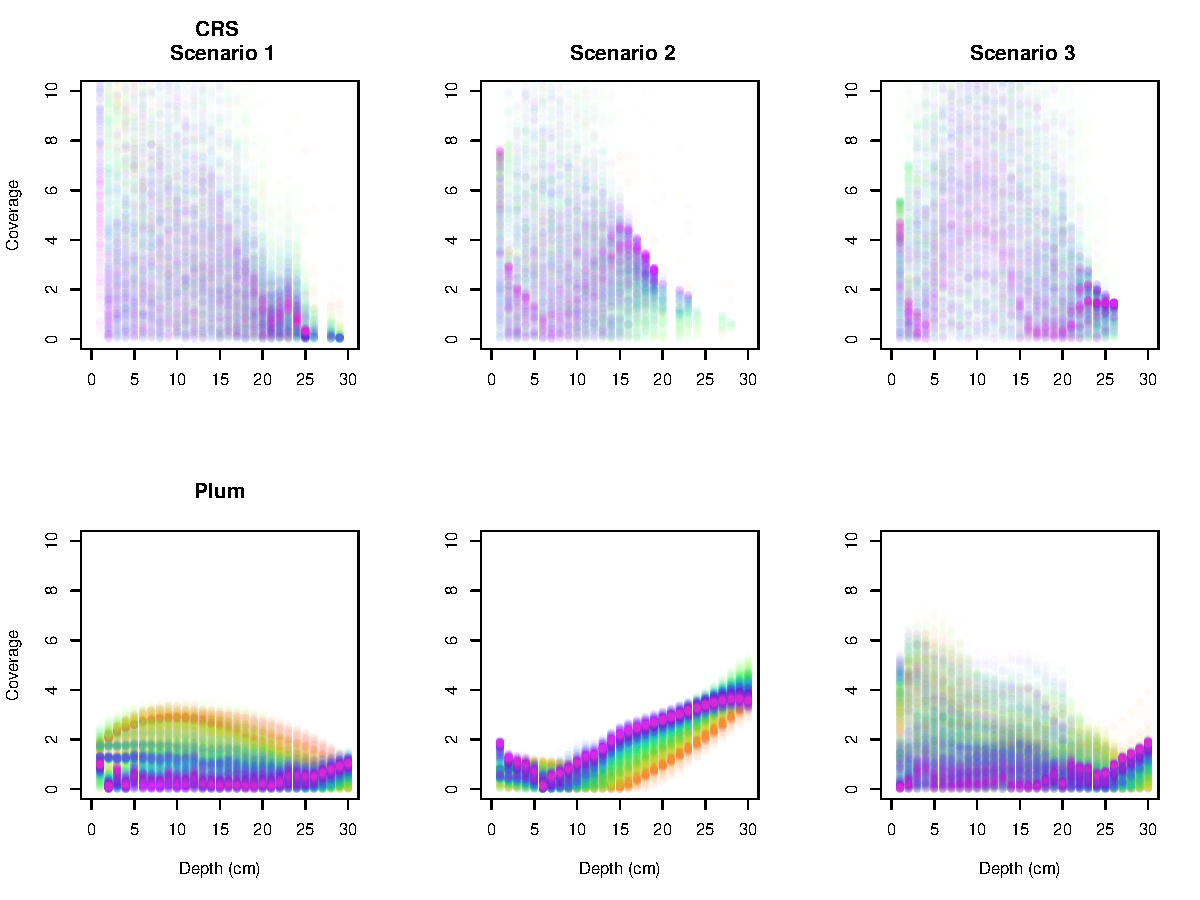
\includegraphics[width=\linewidth]{depthsnew.pdf}
		\caption{Coverage of every sample at every depth for the three simulated scenarios - CI-CRS age estimates at sample depths and \textit{Plum}'s age estimates at 1 cm intervals. Dots go from lowest information percentage samples (few dated depths; red) to high percentage samples (nearly completely dated cores; purple). The CI-CRS's coverage shows no learning pattern at any particular depth regardless of the available information. This means that the model can provide a reasonable chronology with low levels of information or a very inaccurate age estimate with high levels of information at any given depth resulting in an unrealistic age-depth model. On the other hand, \textit{Plum} demonstrates a systematic improvement in its age estimates as more data are available. These results show that \textit{Plum}, as a likelihood based approach, consistently provides more reliable results.   }
		\label{fig:depths}
	\end{centering}
\end{figure}

Figure \ref{fig:depths} shows the coverage of every simulation according to depth for both models.
\textit{Plum} shows a clear learning structure which depends on the information available to the model.
The information percentage appears to be irrelevant to the coverage of the CI-CRS model, contrary to the results obtained by \textit{Plum}.
It is important to note that the inaccuracies of the CI-CRS model are not exclusive to any particular sections of the chronology; this is most likely driven by the small uncertainties estimated by the CI-CRS model.
%See below for a discussion of how \textit{Plum} behaved in sedimentation simulation 2.   



%%%%%%%%%%%%%%%%%%%%%%%%%%%%%%%%%%%%%%%%%%
%%%%%%%%%%%%%%%%%%%%%%%%%%%%%%%%%%%%%%%%%%
\section{Discussion and Conclusions}

This research focuses on exploring the uncertainty and precision of the most commonly used $^{210}$Pb dating methods (CRS, CIC and CF:CS) in contrast to \textit{Plum}.
By using different scenarios, three different simulations were created.
These simulations were then sub-sampled at different percentages of information in order to observe the effects that different sample sizes have on the resulting chronology. 
This experiment provided an objective comparison of the accuracy and precision of both methods.

The experiment was conducted on two levels.
First, we evaluated the overall accuracy and precision of the method.
The mean of the bias, length of the 95\% confidence and credible intervals, as well as the coverage were measured.
Second, we quantified the ability of each model to capture the true value in their credible/confidence interval, and the coverage of each scenario according to depth. 
These two comparisons provided a good picture of the difference in precision and accuracy between these methods.

From the overall accuracy (see Figure \ref{fig:accpre}) it is clear that both the CRS model and \textit{Plum} reduce their bias as more data becomes available, with the Bayesian method providing, on average, a smaller bias regardless of the sample size. 
In terms of precision, the Bayesian method is providing much larger uncertainties when small sample sizes are used. 
It is only with 60\%, or more of information that the length of the intervals becomes comparable. 
This is a consequence of the linear/exponential interpolation between data points used by the CRS method, in contrast to the Bayesian approach (\textit{Plum}).  
As has been previously discussed by \citet{Aquino2020}, the larger uncertainties provided by \textit{Plum} are more realistic, as confirmed in this work.
Further evidence that these uncertainties are more reasonable is that the length of the credible intervals becomes smaller as more data becomes available. 
On the other hand, the length of the confidence intervals provided by the classical model (CRS) remain almost constant at any sample size.
Lastly, the coverage, which shows the ability of the model to capture the true values within their intervals, shows that the classical model (CRS) on average is incapable of capturing the true values within its 95\% confidence interval. 
These results are concerning, considering that the $^{210}$Pb dating community rarely report 95\% confidence intervals and instead tend to use only 65\% confidence intervals (one standard deviation intervals).
On the other hand, \textit{Plum}'s coverages always remain $\leq 2$, therefore guaranteeing that on average the true value is captured within its 95\% credible intervals, even with small sample sizes.
\textit{Plum}'s coverages are constantly improving and reaching stability with 50\% or more of information percentage.
These experiments show that the Bayesian method, on average, provides more reliable results, for both precision and accuracy, no matter the amount of information.


As the coverage demonstrates how well each model can estimate the real value within its intervals, this variable may be used to assess if a certain approach offers a more accurate estimate for various time periods.
Figure \ref{fig:depths} presents the performance of both the CRS model and \textit{Plum} for every simulated scenario.
It appears that the coverage of many of the CRS chronologies are $> 2$ throughout the whole chronology, meaning that the model does not have a period of time for which it is more precise. 
Moreover, the CRS, as applied, does not exhibit a clear learning pattern, where the coverage appears to be indifferent to the amount of information available.
It appears that even high levels of information percentage provide coverages $> 2$, in some cases closer to 4 for scenarios 2 and 3.
\textit{Plum} on the other hand, shows a structure where more data are reflected in improved models in scenarios 1 and 3.
It is only at low levels of information where \textit{Plum}'s coverage is $>2$.
Scenario 2, on the other hand, presents a case where \textit{Plum} is both incapable of capturing the true value, for depths $>15$ cm, and it appears that as more data becomes available the model provides worse results. 
This may be of concern if we do not recognize that this scenario is unrealistic as it presents an extreme change in the accumulation around 15 cm, which coincides with the depth at which the coverage becomes $>2$.
However, it is also important to acknowledge that this experiment was performed using default settings.  
In a real-world scenario the user typically has some prior knowledge of the sedimentation process, about the site of interest, which could be incorporated as prior information to the model to improve the resulting chronology for both the CRS and \textit{Plum} models.

% The results obtained by this experiment appear to persist even in the case of the revised version of the CRS model (R-CRS).
% The R-CRS model appears to improve the bias but this improvement appears to be nullified by the smaller uncertainties presented by \citet{Sanchez-Cabeza2014}.
% The question of which version of the CRS provides the best result is beyond the scope of this research and is dependent on expert application of the model.
% Nevertheless, it is important to note that that the bias, related to the CI-CRS and R-CRS, are reasonably small at certain sections of the sediment, but the uncertainty quantification of both methods is overly optimistic.  

In conclusion, the use of the Bayesian age-depth models is preferred for the consistent construction of sediment chronologies, not only on radiocarbon-based chronologies as presented by \citet{Blaauw2018} but also in the more complex case of $^{210}$Pb shown here.
While the classical approach provides reasonable results regarding the bias, the uncertainty quantification in these methods needs improvement as it does not rely on a proper statistical structure. 
In a real-world scenario, it is impossible to measure the true bias of a method and therefore a proper uncertainty quantification becomes extremely important.
These results support the recommendations presented by \citet{Smith2001,Barsanti2020} where the CRS method, or any dating methodology, should be validated using independent dating markers. 

Lastly, it is important to highlight the benefits of the Bayesian methods.
From both \citet{Blaauw2018} and the present work, it is shown that Bayesian methods constantly improve as more data are added, and the uncertainty associated to the method is realistic and coherent with the amount of information available. 
This leads to chronologies that are capable of capturing the true age in their credible intervals, especially with minimal expert input (unlike the CRS which relies on expert modifications). 
The ability to capture the true value in the credible intervals becomes important when the problem is associated with decision making processes, as it provides a more realistic picture of the available knowledge of the process. 
Given that $^{210}$Pb-dating is now widely used in pollution, environmental and climate change studies, which potentially have a high impact on both policy-making and public perception, realistic age estimates and uncertainties become extremely important.

\section{Acknowledgments}

The authors are partially funded by CONACYT CB-2016-01-284451 and COVID19 312772 grants and a RDCOMM grant.
The corresponding author is funded by CONACYT through the postdoctoral residence program with CVU  489201.


\bibliographystyle{apalike}
\bibliography{bibliography.bib}
\newpage


% \section{Supplementary Material}
% \label{sec:supp_mat}
% Data for each simulation and code used are hosted at: \url{https://github.com/maquinolopez/Paper_Simulations}

% \section{Appendix A}

% Bias, length of 95\% confidence intervals (credible intervals for \textit{Plum}) and coverage of the CIC and CF:CS models are shown in Figure \ref{fig:CIC-CFCS}.
% As can be observed and as expected the bias of the CIC model (which can be considered the simplest model) is much bigger when compared to any other alternative and it does not decrease as more data are available.
% The confidence interval remains the same regardless of the information available, and coverage is almost always above two, which means that the uncertainties are not sufficient to capture the true age-depth model.
% On the other hand the CF:CS model does decrease its bias as more data are available and after 60\% to 70\% this decrease does not seen improve.
% The length of the interval remains the same regardless of the information available and the coverage just like the CIC model is almost always above 2 meaning that the uncertainties are not sufficient.

% These results are consistent with the discussion in the paper as classical model appear to not improve as more data are available.
% Its bias does decrease as more data are available (in the case of the CF:CS model) but its uncertainty is underestimated which in turn does not allow the method to have a reasonable coverage. 


% \begin{figure}
% 	\begin{centering}
% 		\includegraphics[width = 13cm]{AccPrec-appendix.pdf}
% 		\caption{ Top panel A) shows the bias between the modelled and true age of the CF:CS (purple) and CIC (Orange). Middle panel B) shows the 95\% confidence intervals (credible intervals for \textit{Plum}). Bottom panel C) shows the coverage, presenting the distance between the modelled age and the true age divided by the standard deviation. }
% 		\label{fig:CIC-CFCS}
% 	\end{centering}
% \end{figure}

\end{document}
